\chapter{Mesures}

\setlength{\parindent}{0pt}
\renewcommand{\labelitemi}{\textbullet} % Utiliser des points noirs (•)

% ==================================================================================================================================
% Définitions et généralités

\section{Définitions et généralités}

Soit $(X, \B)$ un espace mesurable.

\begin{definition}[Mesure]
    Une fonction sur $(X, \B)$ $ \mu : \B \longrightarrow \overline{\R_+} $ telle que :
    \begin{enumerate}
        \item $\mu (\emptyset) = 0 $
        \item $ \forall (A_n)_{n\in\N}$ suites de parties mesurables deux à deux disjointes :
            \[ \mu \left( \bigcup_{n\in\N} A_n \right) = \sum_{n=0}^{\infty} \mu (A_n) \]
    \end{enumerate}
    est appelée \textbf{mesure} sur l'espace $(X,\B,\mu)$, alors appelé espace mesuré.
\end{definition}

\begin{example}[Mesure de Comptage]
    Soient $X$ un ensemble et $\mathcal{B} = \mathcal{P}(x)$. On définit alors :
        \[ c :
            \begin{cases}
                \mathcal{P}(X) \longrightarrow \overline{\R_+} \\
                A \longmapsto \begin{cases}
                                    \infty \text{ si } A \text{ est infini }
                                    |A| \text{ sinon }
                                \end{cases}
            \end{cases}
        \] 
    est une mesure nommé \textbf{mesure de comptage}.
\end{example}

\begin{prop}[Mesures]
    Soit $(X,\B,\mu)$ un espace mesuré et $\mu$ sa mesure. Elle vérifie les propriétés suivantes :
    \begin{itemize}
        \item \textbf{Croissance :} La mesure est une fonction croissante i.e 

            \begin{minipage}{0.3\textwidth}
                \begin{tikzpicture}[scale=0.6]
                    % Dessin de l'ensemble B
                    \draw[thick] (-2,0) ellipse (3 and 2); % Patatoïde pour B
                
                    % Dessin de l'ensemble A (à l'intérieur de B)
                    \begin{scope}
                        \clip (-1.5,0) ellipse (2 and 1.5); % Clip pour hachurage uniquement dans A
                        \fill[pattern=north west lines, pattern color=gray] (-2,0) ellipse (3 and 2); % Hachurage de A
                    \end{scope}
                    \draw[thick] (-1.5,0) ellipse (2 and 1.5); % Contour de A
                
                    % Annotations
                    \node at (-3,1.5) {$B$};           % Annotation de B
                    \node at (-1.5,1) {$A$};           % Annotation de A
                    \node at (-4, -1) {$A \setminus B$}; % Annotation pour la partie A privé de B
                \end{tikzpicture}
            \end{minipage}%
            \hfill
            \begin{minipage}{0.55\textwidth}  % Largeur pour le texte
                $\forall A,B \in \B$ tels que  $A \subseteq B,$ on a  
                \begin{itemize}
                    \item  $\mu(A) \leq \mu (B)$
                    \item $\mu(B) = \mu(A) + \mu (B \setminus A)$
                \end{itemize}
            \end{minipage}

        \item \textbf{Convergence par union croissante :} Soit $(A_n)_{n\in\N}$ une suite croissante de parties mesurables
            \[ \text{ i.e } \forall n \in \N, A_n \subseteq A_{n+1}, \text{ alors } \mu \left( \bigcup_{n\in\N} A_n \right) = \lim_{n\to\infty} \mu(A_n) \] 
        \item \textbf{Convergence par intersection décroissante :} Soit $(A_n)_{n\in\N}$ une suite décroissante de parties mesurables de mesure finie
            \[ \text{ alors } \mu \left( \bigcap_{n\in\N} A_n \right) = \lim_{n\to\infty} \mu (A_n) \] 
    \end{itemize}
\end{prop}

\begin{definition}[Mesure Induite]
    Soit $A \subseteq C$ où $(X,\B,\mu)$ est un espace mesuré. On munit $A$ d'une structure d'espace mesuré $(A, \B_{\restriction _A}, \mu_A)$ où $\B_{\restriction _A}$ est la tribu induite.
    Alors $\mu_A$ est appelée mesure induite.
\end{definition}

\begin{definition}[Mesure Pondéré]
    Soit $\omega \in \mathcal{M}_+(X)$ et $(X, \mathcal{B},\mu)$ un espace mesuré. 

    Posons : $$ \mu_\omega = \omega \mu \quad \text{ où } \quad \mu_\omega : A \longmapsto \int_A \omega \; d \mu $$

    $\mu_\omega$ est alors appelée mesure pondérée par $\omega$. On a donc : 
        \[ f \in (X, \mathcal{B},\mu_\omega) \; \iff \; f \omega \in (X, \mathcal{B},\mu) \] 
\end{definition}

\section{Mesure de Lebesgue sur les réels}

\begin{theorem}[Existence de la mesure de Lebesgue]
    Il existe une unique mesure sur $(\R, \B_\R)$ notée $\lambda$ telle que :
        \[ \boxed{ \forall a,b \in \R, a \leq b, \quad \lambda(]a,b]) = b-a } \] 
    Cette mesure est appelée \textbf{mesure de Lebesgue}. En partiulier, on a $ \lambda (\R) = \infty $ 
\end{theorem}

\begin{remark}
    $\lambda (\R) = \infty$ car :
        \[ R = \bigcup_{n \in \N} ]-n, n[ \text{ donc } \lambda (\R) = \lambda \Big( \bigcup_{n \in \N} ]-n, n[ \Big) = \lim_{n\to\infty} (2n) = \infty \] 
\end{remark}

\section{Parties négligeables et ensemble de Cantor}

\begin{definition}[Parties négligeables]
    Soit $A \in \B$ une partie mesurable, on dit que $A$ est une \textbf{partie néligable} ssi $\lambda (A) = 0 $.
    On dit aussi que $B \in \B$ est une \textbf{partie pleine} ssi $\lambda(B ^c) = 0 $.  On remarquera que toute partie dénombrable est négligeable.
\end{definition}

\begin{proof}
    Soit $A$ une partie dénombrable. On a $A = \bigcup_{x\in A} \{ x \}$ d'où :
        \[ \lambda (A) = \lambda \left( \bigcup_{x\in A} \{ x \} \right) = \lambda(x_1) + \dots + \lambda(x_n) = 0 \]
\end{proof}

\textbf{(?)} Existe-t-il une partie négligeable non dénombrable ?

\begin{example}[Ensemble de Cantor]
    Soit $(C_n)_{n\in N}$ une suite de fermés non vides décroissante. Posons $C = \bigcap_{n\in N} C_n$ un fermé non vide.
        \[ \text{Alors :  } \lambda (C) = \left( \frac{2}{3} \right) ^n \underset{n\to\infty}{\longrightarrow} 0 \]
    $C$ est donc négligeable mais on peut montrer que $C$ est en bijection avec $\{0,2\}^\N \simeq \R$ qui n'est pas dénombrable.
    Donc $C$ n'est pas dénombrable.

    \centering
    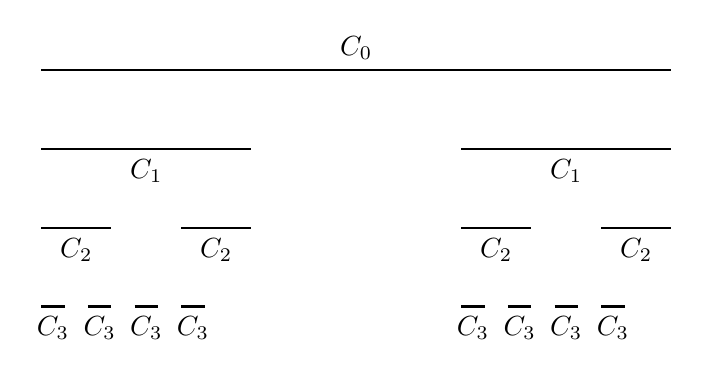
\begin{tikzpicture}[scale=1]
        % Définir la longueur initiale
        \def\length{8}
        \def\height{1}
        % Dessiner la première ligne (niveau 0)
        \draw[thick] (0, 0) -- (\length, 0) node[midway, above] {$C_0$};
        % Dessiner les lignes des niveaux suivants
        % Niveau 1
        \draw[thick] (0, -\height) -- (2.6667, -\height) node[midway, below] {$C_1$}; % 8/3
        \draw[thick] (5.3333, -\height) -- (8, -\height) node[midway, below] {$C_1$}; % 8/3
        % Niveau 2
        \draw[thick] (0, -2*\height) -- (0.8889, -2*\height) node[midway, below] {$C_2$}; % 8/9
        \draw[thick] (1.7778, -2*\height) -- (2.6667, -2*\height) node[midway, below] {$C_2$}; % 8/9
        \draw[thick] (5.3333, -2*\height) -- (6.2222, -2*\height) node[midway, below] {$C_2$}; % 8/9
        \draw[thick] (7.1111, -2*\height) -- (8, -2*\height) node[midway, below] {$C_2$}; % 8/9
        % Niveau 3
        \draw[thick] (0, -3*\height) -- (0.2963, -3*\height) node[midway, below] {$C_3$}; % 8/27
        \draw[thick] (0.5926, -3*\height) -- (0.8889, -3*\height) node[midway, below] {$C_3$}; % 8/27
        \draw[thick] (1.1852, -3*\height) -- (1.4815, -3*\height) node[midway, below] {$C_3$}; % 8/27
        \draw[thick] (1.7778, -3*\height) -- (2.0741, -3*\height) node[midway, below] {$C_3$}; % 8/27
        \draw[thick] (5.3333, -3*\height) -- (5.6296, -3*\height) node[midway, below] {$C_3$}; % 8/27
        \draw[thick] (5.9259, -3*\height) -- (6.2222, -3*\height) node[midway, below] {$C_3$}; % 8/27
        \draw[thick] (6.5185, -3*\height) -- (6.8148, -3*\height) node[midway, below] {$C_3$}; % 8/27
        \draw[thick] (7.1111, -3*\height) -- (7.4074, -3*\height) node[midway, below] {$C_3$}; % 8/27
    \end{tikzpicture}
\end{example}

\begin{definition}[Presque Partout]
    Une propriété $\mathcal{P}(X)$ qui dépend d'une variable $X$ variant dans une espace mesuré $(X,\B,\mu)$ est dite vraie "presque partout", noté (p.p) si 
        \[ \{ x \in X : \lnot \mathcal{P}(X) \} \text{ est négligeable } \] 
\end{definition}

\begin{example} Exemples de parties négligeables et propriétés vraies presque partout :
    \begin{itemize}
        \item  Soient $f,g \in \overline{\M_+(X)}$, on a :
            \[ f = g \text{ presque partout } \quad \Longleftrightarrow \quad \mu(\{x \in X : f(x) = g(x) \}) = 0 \] 
        \item $\mathbb{1}_\Q = 0$ p.p car $\Q$ est négligeable et $\R \backslash \Q$ est une partie pleine. 
    \end{itemize}
   
\end{example}
